\appendix
\addcontentsline{toc}{chapter}{Appendices}
\startcontents
\startlist[appendix]{lof}
\startlist[appendix]{lot}
\printcontents{atoc}{0}{\chapter*{Appendices}}
\begingroup
\let\clearpage\relax
\singlespacing
\printlist[appendix]{lof}{}{\chapter*{List of Figures}}
\printlist[appendix]{lot}{}{\chapter*{List of Tables}}
\endgroup

\chapter{Appendices}
\label{app:Appendix}

\section{Additional tables}

\subsection{Chapter 4 Tables}

\begin{table}[htbp]
%\setlength{\tabcolsep}{20pt} only to stretch the columns if you want
%\renewcommand{\arraystretch}{1.5}
\centering
\begin{tabular}{@{} c c c}
\toprule
\textbf{Sample ID} & \textbf{NRF} & \textbf{PBC1/PBC2} \\
\midrule
\midrule
PS2000 CD14	& 76.0	& \\
PS2001 CD14	& 83.2	& \\
PS2314 CD14	& 79.6	& \\
PS2319 CD14	& 78.2	& \\
CTL7 CD14	  & 79.4	& \\
CTL8 CD14	  & 82.4	& \\
CTL9 CD14	  & 79.2	& \\
CTL10 CD14	& 81.5	& \\
\midrule
PS2000 CD4  & 83.3	& \\
PS2001 CD4	& 80.6	& \\
PS2314 CD4	& 81.3	& \\
PS2319 CD4	& 80.8	& \\
CTL7 CD4	  & 76.8	& \\
CTL8 CD4    & 80.1	& \\
CTL9 CD4    & 80.0	& \\
CTL10 CD4   & 76.1	& \\
\midrule
PS2000 CD8 & 75.9 &	\\
PS2001 CD8 & 72.8 &	\\
PS2314 CD8 & 72.4 &	\\
PS2319 CD8 & 70.7 &	\\
CTL7 CD8	 & 31.8 &\\
CTL8 CD8	 & 68.2 &	\\
CTL9 CD8	 & 72.1 &	\\
CTL10 CD8	 & 66.1 &	\\
\midrule
PS2000 CD19	& 36.9 &\\
PS2001 CD19	& 70.2 &\\
PS2314 CD19	& 28.4 &	\\
PS2319 CD19	& 74.4 &	\\
CTL7	CD19  & 72.3	&\\
CTL8	CD19  & 66.7  &	\\
CTL9	CD19  & 73.3  &	\\
CTL10	CD19  & 60.1  &\\
\bottomrule
\end{tabular}
\medskip %gap
\caption[Evaluation of ChiPm library complexity for the psoriasis and control chort 1B ChIPm assay.]{\textbf{Evaluation of ChiPm library complexity for the psoriasis and control chort 1B ChIPm assay.} NRF, PBC1 and PBC2 are the three measures used according to the ENCODE standards as referred in Chapter \ref{ch:Mat}. 0.5$\leq$NRF$<$0.8 acceptable; 0.8$\leq$NRF$\leq$0.9 compliant; NRF$>$0.9 ideal; PBC1$>$0.8 and PBC2$\geq$10 no bottlenecking.}
\label{tab:ChIPm_PS_CTL_library_complexity}
\end{table}
\bigskip %bigger space



\subsection{Chapter 5 Tables}

\begin{table}[htbp]
%\setlength{\tabcolsep}{20pt} only to stretch the columns if you want
%\renewcommand{\arraystretch}{1.5}
\centering
\begin{tabular}{@{} c }
\toprule
\textbf{CC-mixed CD14$+$ monocytes additional enriched pathways} \\
\midrule
\midrule
SLE \\
Translation \\
3'-UTR-mediated translational regulation \\
Th1 and Th2 cell differentiation \\
Peptide chain elongation \\
Rheumatoid arthritis \\
Metabolism of proteins \\
Cell adhesion molecules (CAMs) \\
Th17 cell differentiation \\
Nonsense Mediated Decay Enhanced by the Exon Junction Complex \\
SRP-dependent co-translational protein targeting to membrane \\
Hemostasis \\
Metabolism of mRNA \\
Platelet activation, signalling and aggregation \\
HTLV-I infection \\
Innate immune system \\
Adaptive immune system \\
\bottomrule
\end{tabular}
\medskip %gap
\caption[Additional enriched pathways for the genes differentially expressed between SF and PB CD14$^+$ monocytes from the CC-mixed subpopulation.]{\textbf{Additional enriched pathways for the genes differentially expressed between SF and PB CD14$^+$ monocytes from the CC-mixed subpopulation.} All the enriched pathways contained a minimum of ten DEGs from the analysis and were significant at an FDR$<$0.01.}
\label{tab:PSA_scRNAseq_CC_mixed_additional_pathways}
\end{table}


\begin{table}[htbp]
%\setlength{\tabcolsep}{20pt} only to stretch the columns if you want
%\renewcommand{\arraystretch}{1.5}
\centering
\begin{tabular}{@{} c }
\toprule
\textbf{CC-IL7R CD14$+$ monocytes additional enriched pathways} \\
\midrule
\midrule
SLE \\
Tuberculosis \\
Epstein-Barr virus infection \\
Immune System \\
\bottomrule
\end{tabular}
\medskip %gap
\caption[Additional enriched pathways for the genes differentially expressed between SF and PB CD14$^+$ monocytes from the CC-mixed subpopulation.]{\textbf{Additional enriched pathways for the genes differentially expressed between SF and PB CD14$^+$ monocytes from the CC-IL7R subpopulation.} All the enriched pathways contained a minimum of five DEGs from the analysis and were significant at an FDR$<$0.01.}
\label{tab:PSA_scRNAseq_CC_IL7R_additional_pathways}
\end{table}

%

\section{Additional figures}
\subsection{Chapter 3 Figures}
\begin{figure}[htbp]
\centering
\begin{subfigure}{0.70\textwidth}
\centering
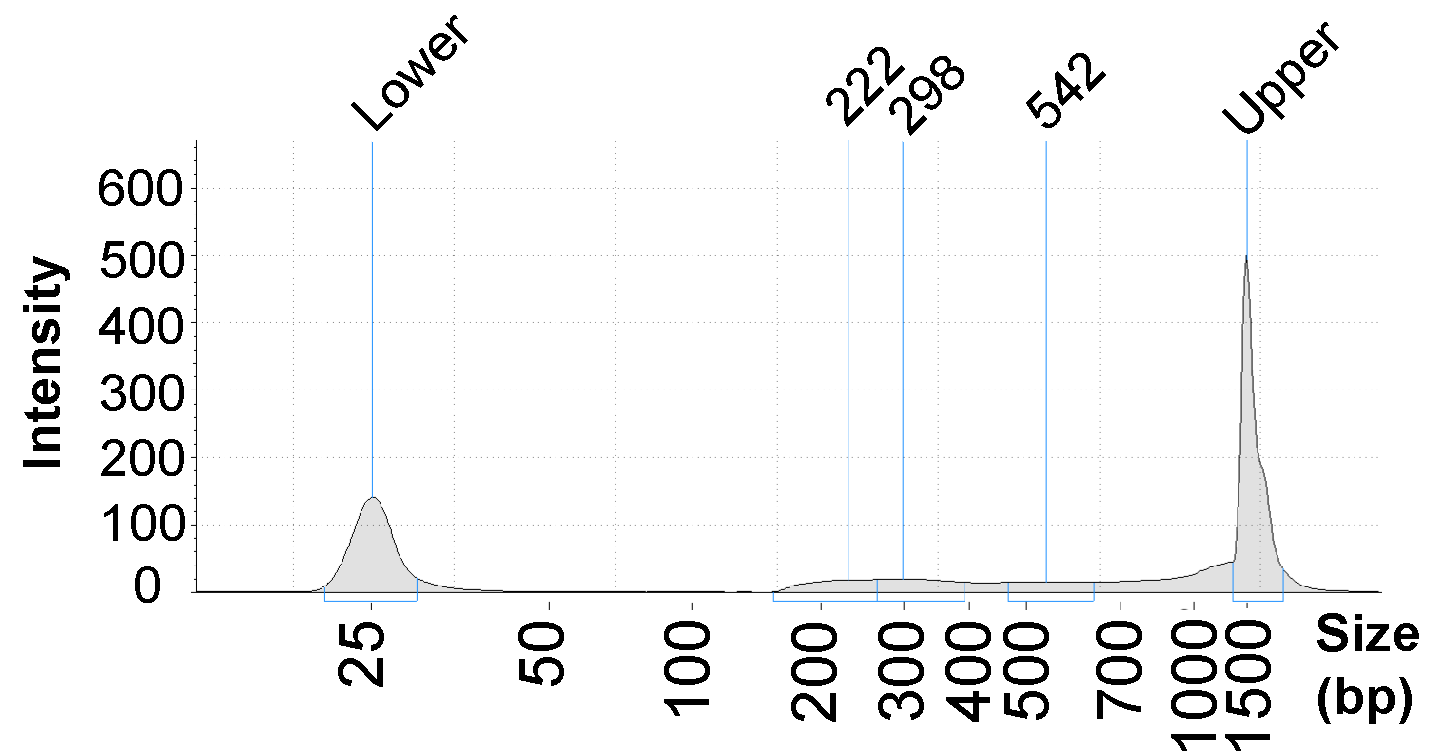
\includegraphics[width=\textwidth]{./Appendix/pdfs/Chapter3/FAST_ATAC_skin_tapestation_C1}
\caption{\textbf{}}
% The percentage sign indicated that the other subfig goes side by side
\end{subfigure}
\begin{subfigure}{0.70\textwidth}
\centering
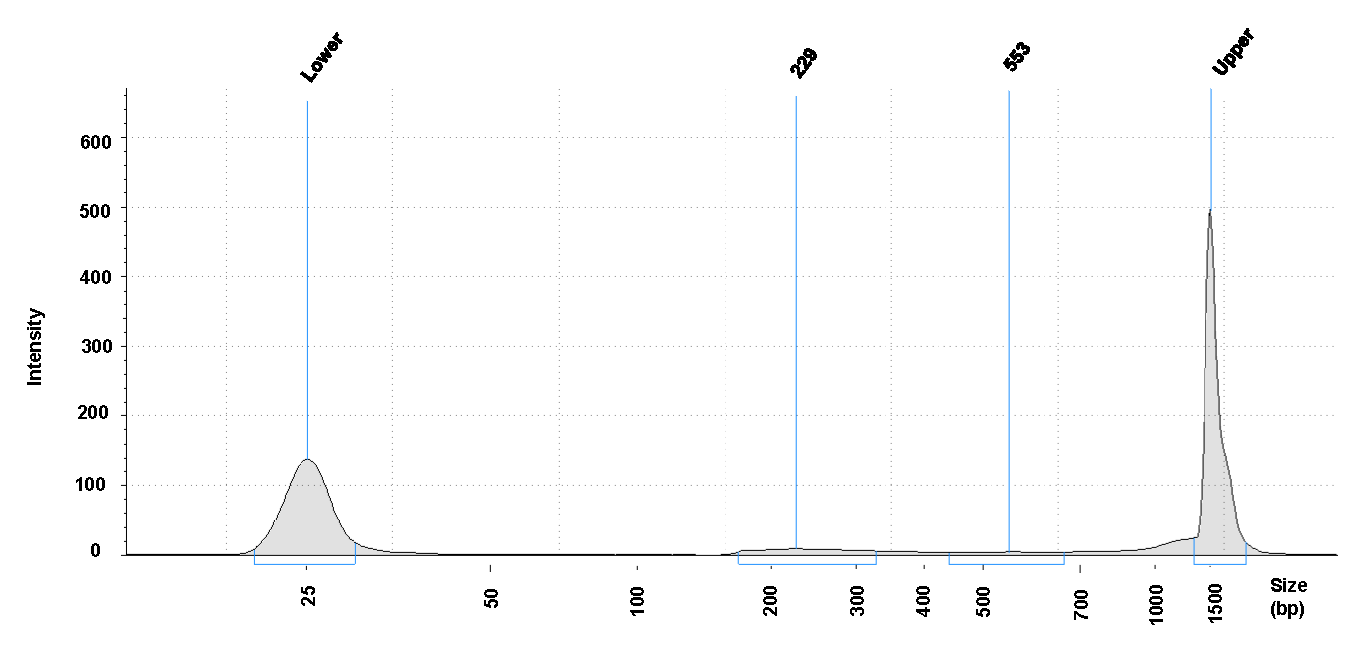
\includegraphics[width=\textwidth]{./Appendix/pdfs/Chapter3/FAST_ATAC_skin_tapestation_C3}
\caption{\textbf{}}
\end{subfigure}
\begin{subfigure}{0.70\textwidth}
\centering
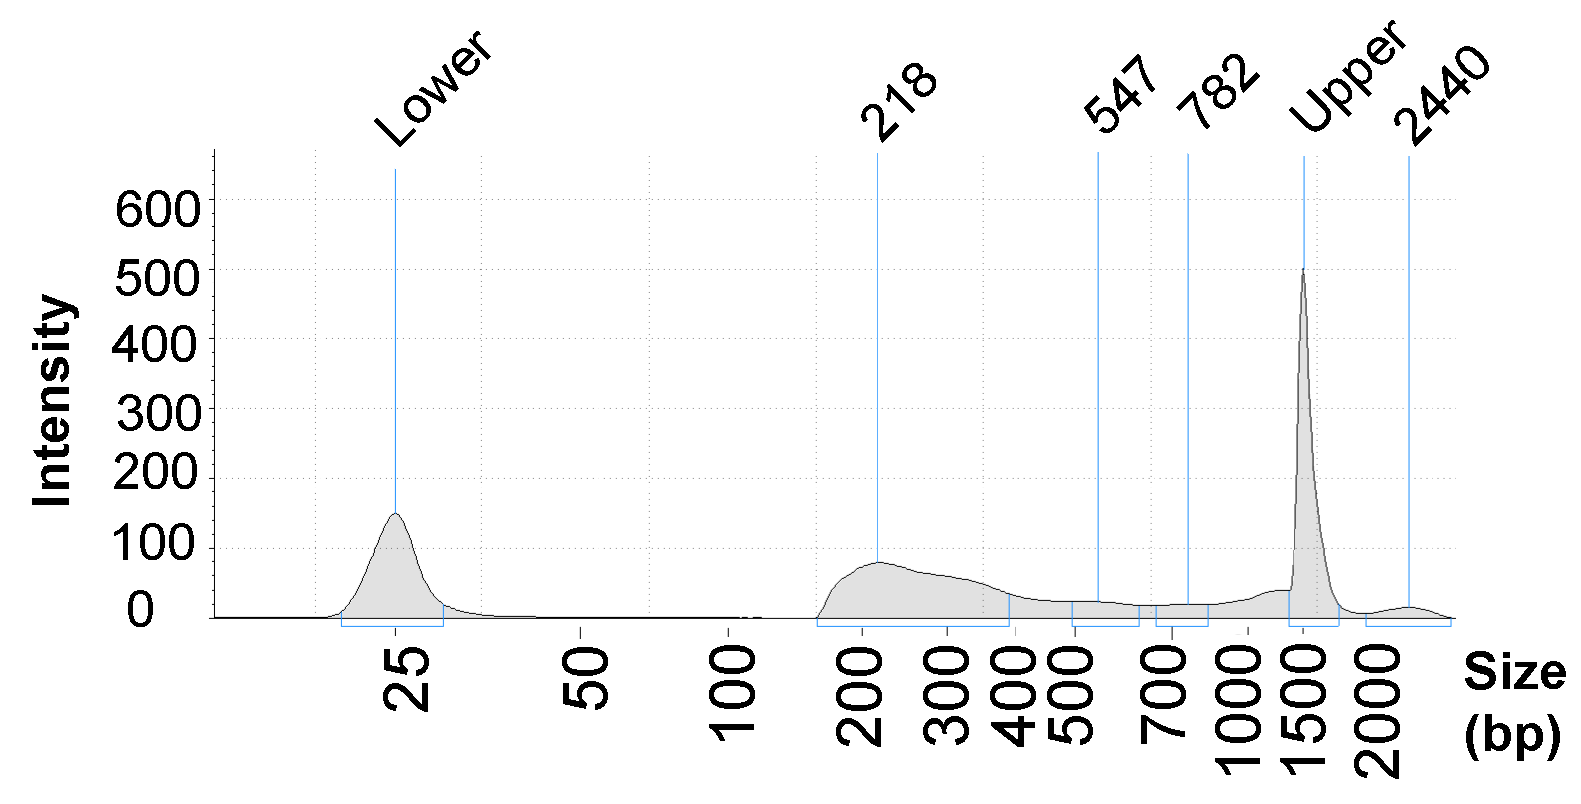
\includegraphics[width=\textwidth]{./Appendix/pdfs/Chapter3/FAST_ATAC_skin_tapestation_C4}
\caption{\textbf{}} % to add text to the figure name
\end{subfigure}
\begin{subfigure}{0.70\textwidth}
\centering
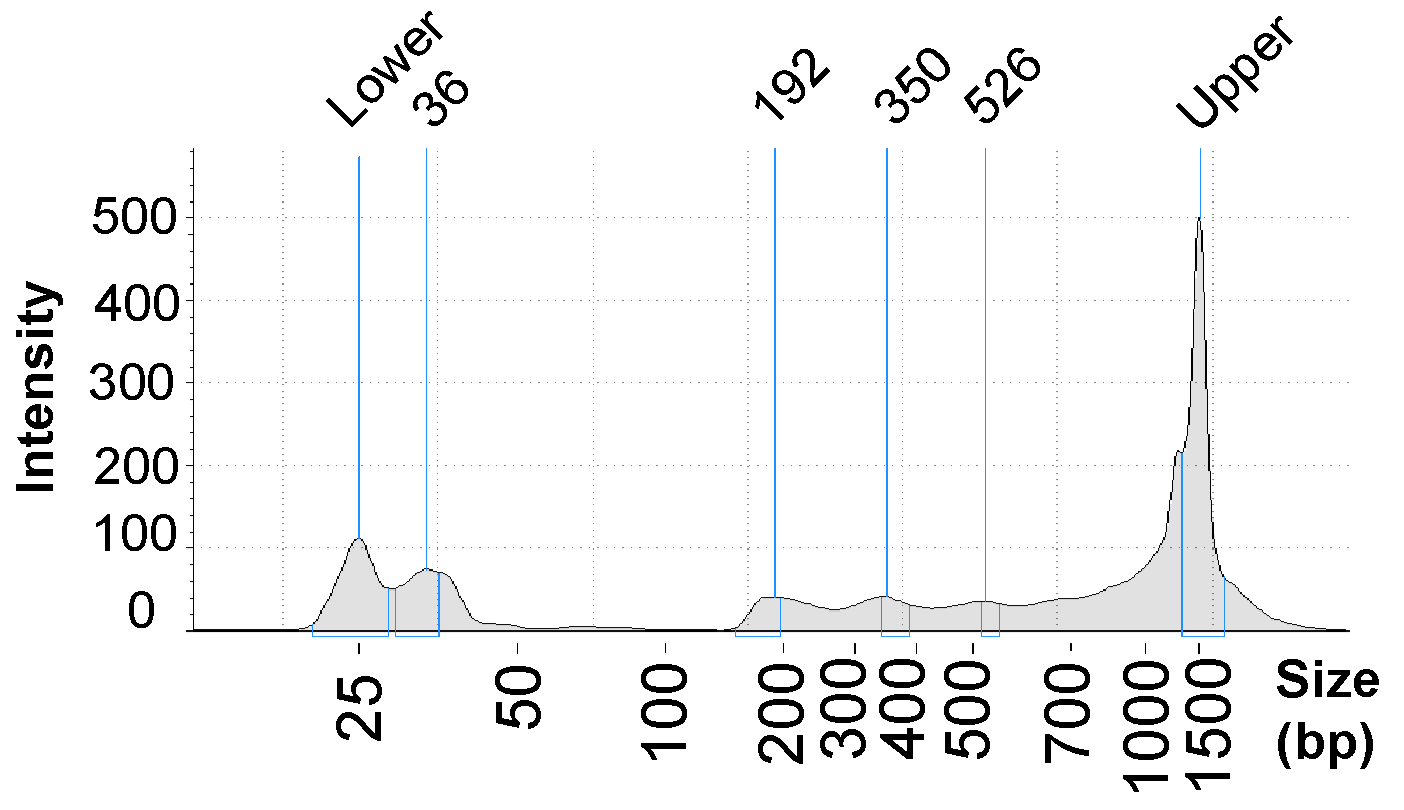
\includegraphics[width=\textwidth]{./Appendix/pdfs/Chapter3/Omni_ATAC_NHEK_Rep1_tapestation}
\caption{\textbf{}} % to add text to the figure name
\end{subfigure}
\hfill
\caption[FAST-ATAC and Omni-ATAC NHEK tapestation profiles.]{\textbf{FAST-ATAC and Omni-ATAC NHEK tapestation profiles.} \\
}
\label{fig:NHEK_tapestation}
\end{figure}



\begin{figure}[htbp]
\centering
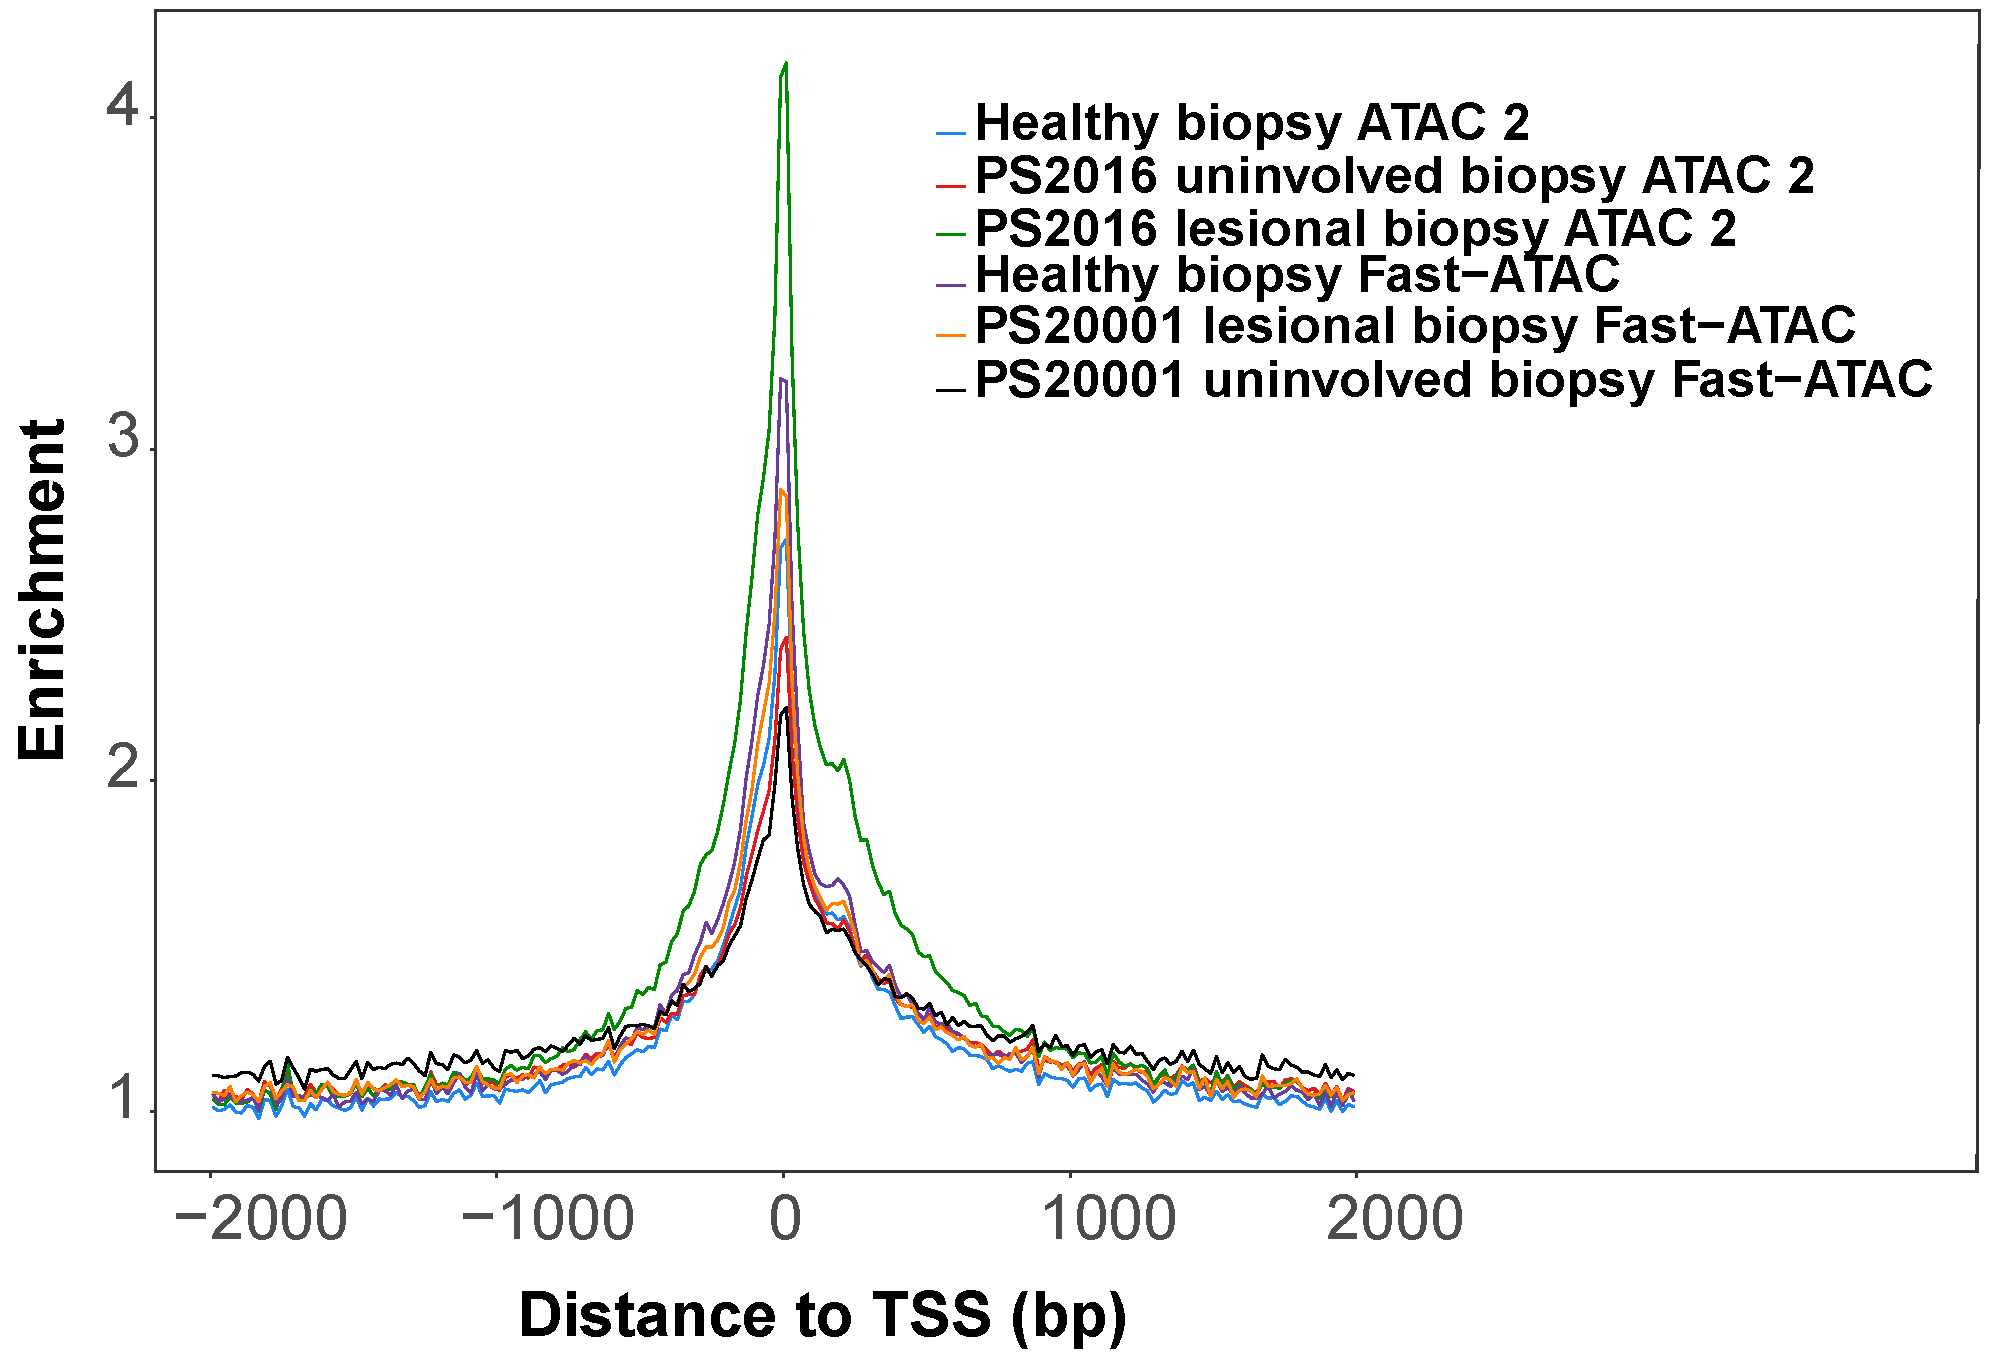
\includegraphics[width=0.8\textwidth]{./Appendix/pdfs/Chapter3/ATAC_skin_biopsy_samples_all_methods_TSS_enrichment_supplementary}
\caption[Assessment of TSS enrichment from ATAC-seq and FAST-ATAC in healthy and psoriasis skin biopsies samples.]{\textbf{Assessment of TSS enrichment from ATAC-seq and FAST-ATAC in healthy and psoriasis skin biopsy samples.}  }
\label{fig:TSS_skin_biopsies}
\end{figure}



\subsection{Chapter 5 Figures}

\bigskip
\begin{figure}[H]
\centering
\begin{subfigure}[b]{0.45\textwidth}
\centering 
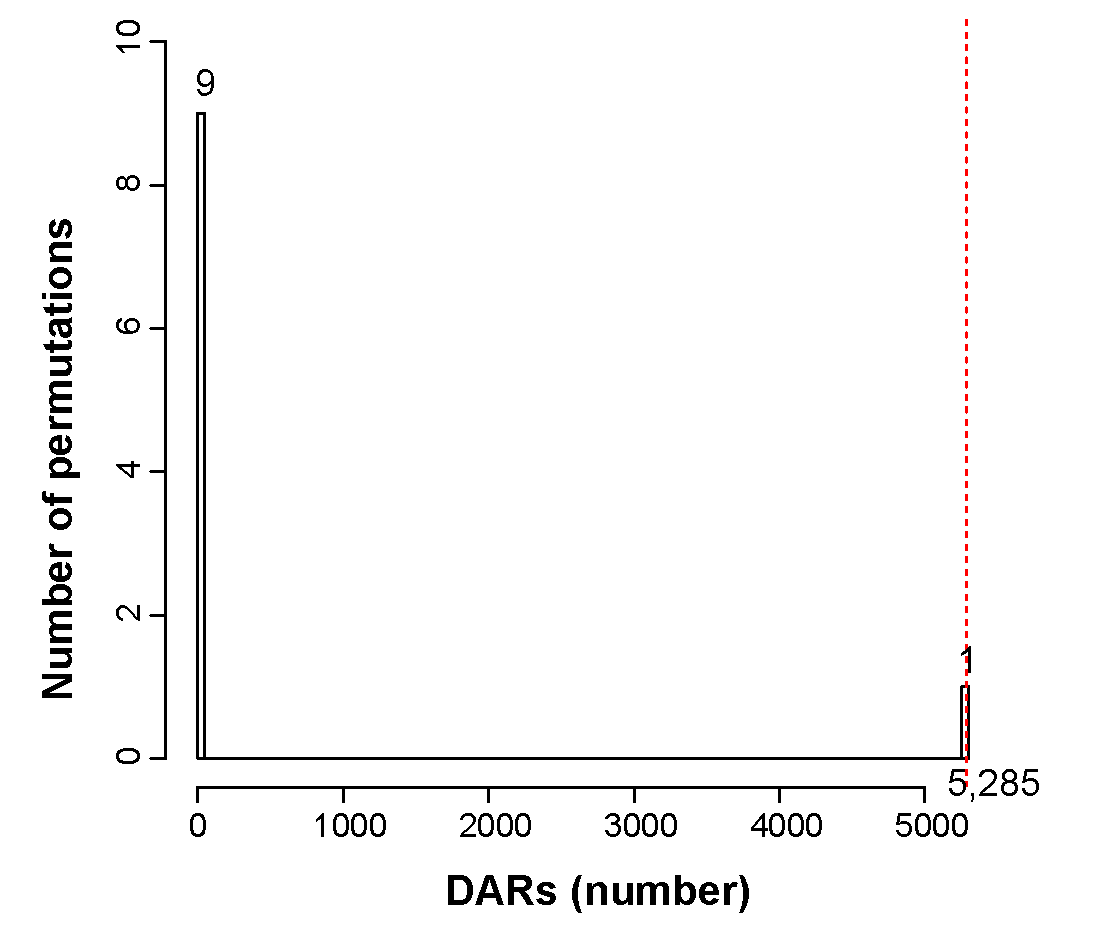
\includegraphics[width=\textwidth]{./Appendix/pdfs/Chapter5/ATAC_PsA_CD14_permutation_analysis}
\caption{}
\end{subfigure}
~
\begin{subfigure}[b]{0.45\textwidth}
\centering 
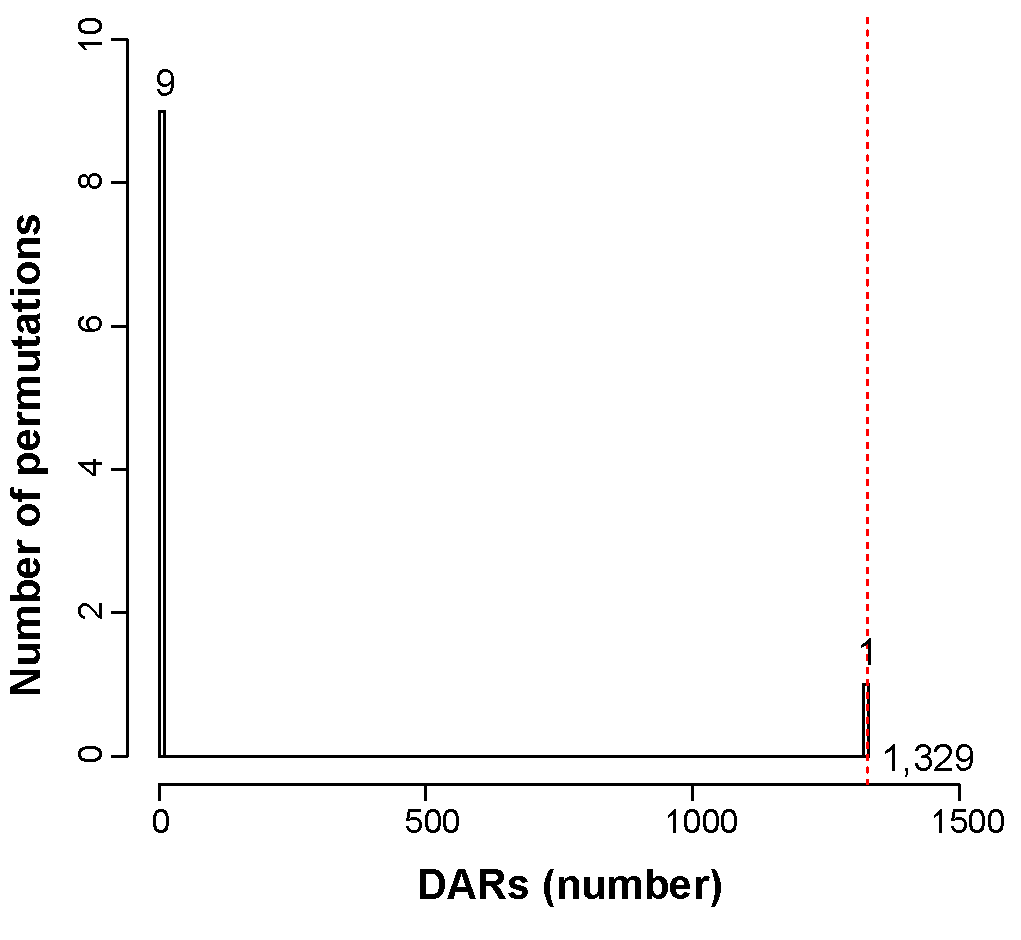
\includegraphics[width=\textwidth]{./Appendix/pdfs/Chapter5/ATAC_PsA_CD4_permutation_analysis}
\caption{}
\end{subfigure}
~
\begin{subfigure}[b]{0.45\textwidth} 
%the [b] prevents offset in subcaptions
\centering
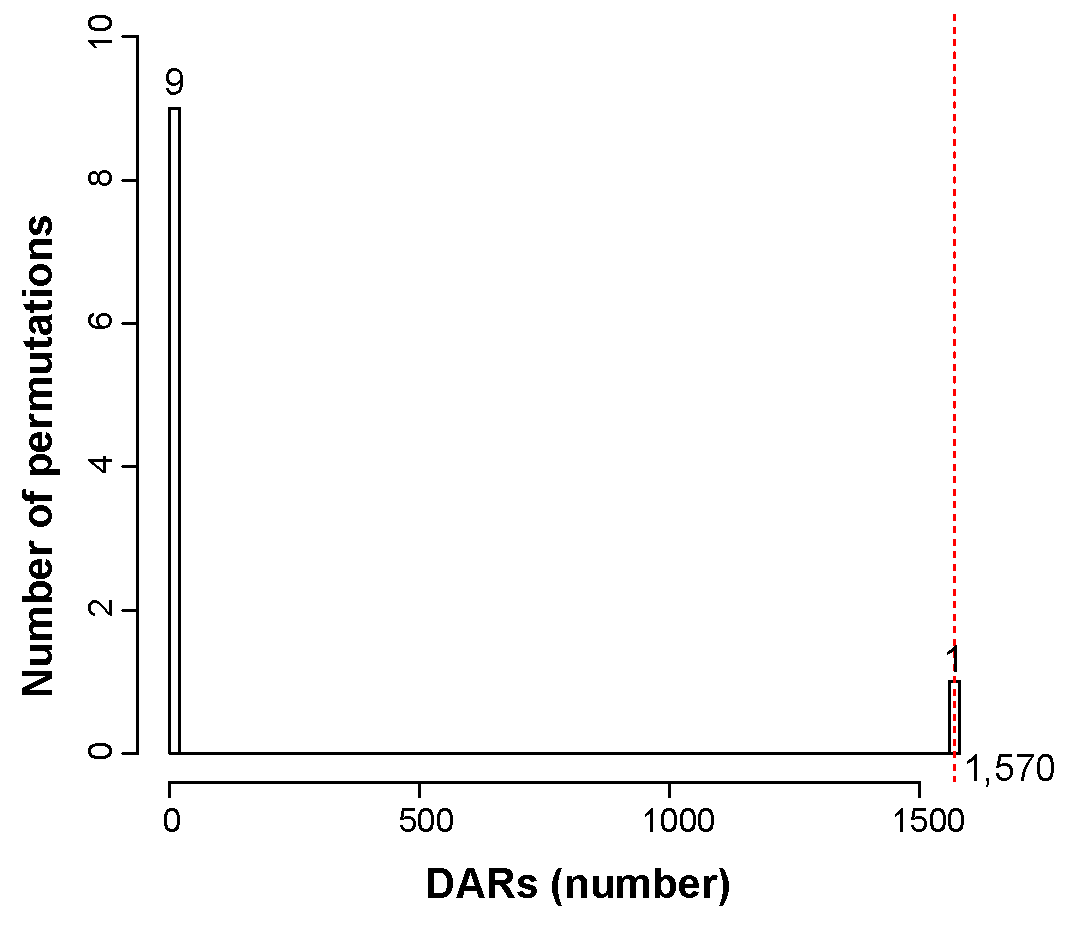
\includegraphics[width=\textwidth]{./Appendix/pdfs/Chapter5/ATAC_PsA_CD8_permutation_analysis}%
\caption{}
\end{subfigure}
\begin{subfigure}[b]{0.45\textwidth} 
%the [b] prevents offset in subcaptions
\centering
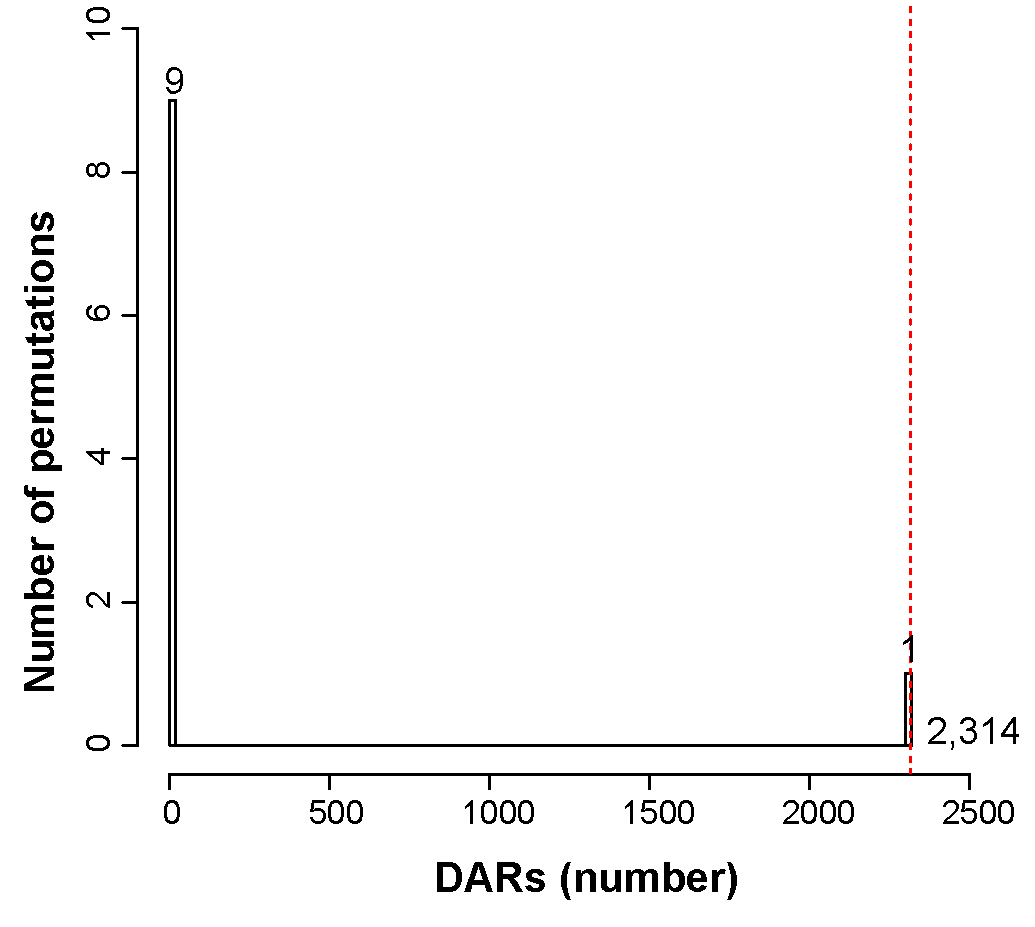
\includegraphics[width=\textwidth]{./Appendix/pdfs/Chapter5/ATAC_PsA_NK_permutation_analysis}%
\caption{}
\end{subfigure}
\caption[Permutation analysis SF vs PB in CD14$^+$,CD4m$^+$,CD8m$^+$ and NK.]{\textbf{Permutation analysis SF vs PB in CD14$^+$,CD4m$^+$,CD8m$^+$ and NK}. }
\label{figure:PsA_perm_analysis}
\end{figure}

\begin{figure}[htbp]
\centering
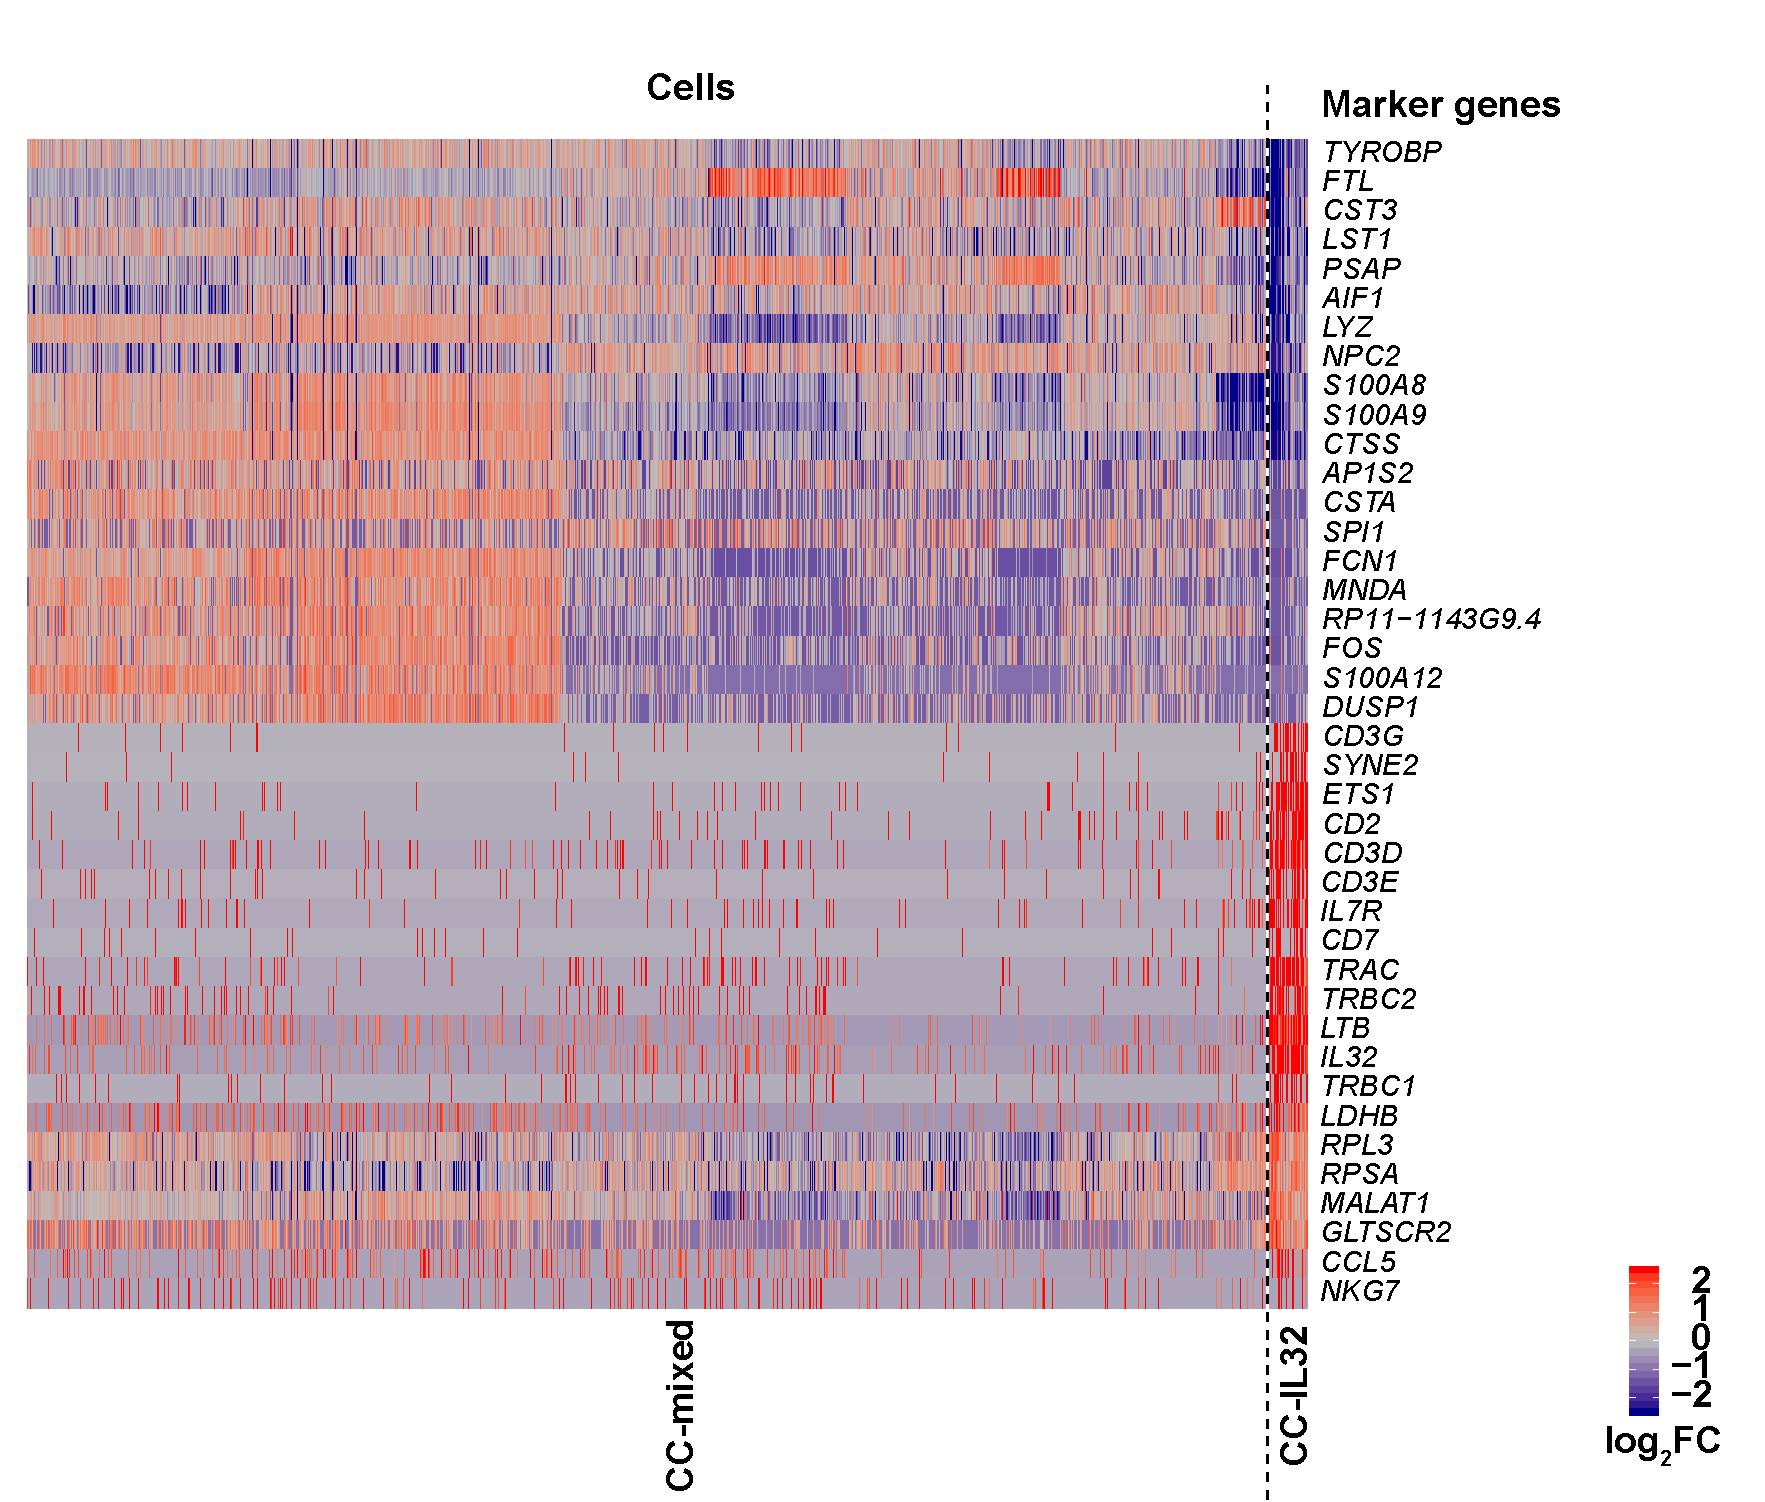
\includegraphics[width=0.6\textwidth]{./Appendix/pdfs/Chapter5/PSA_10X_heatmap_SF_PB_monocytes_clusters_mixed_and_IL7R}
\caption[Heatmap for the top 20 marker genes of the CC-mixed and CC-IL7R CD14$^+$ monocytes subpopulations.]{\textbf{Heatmap for the top 20 marker genes of the CC-mixed and CC-IL7R CD14$^+$ monocytes subpopulations.} Rows are the top 20 marker genes for each of the two subpopulations (total of 40 genes). The columns represent each of the cells members of the CC-mixed (left) or CC-IL7R (right) clusters. The colour scale represents the log$_2$FC in the expression of the marker gene in a particular cell of the cluster compared to the average expression of all the cells from the other cluster.}
\label{fig:PSA_scRNAseq_CC_mixed_and_IL7R_markers_heatmap}
\end{figure}

\bigskip
\begin{figure}[H]
\centering
\begin{subfigure}[b]{0.70\textwidth}
\centering 
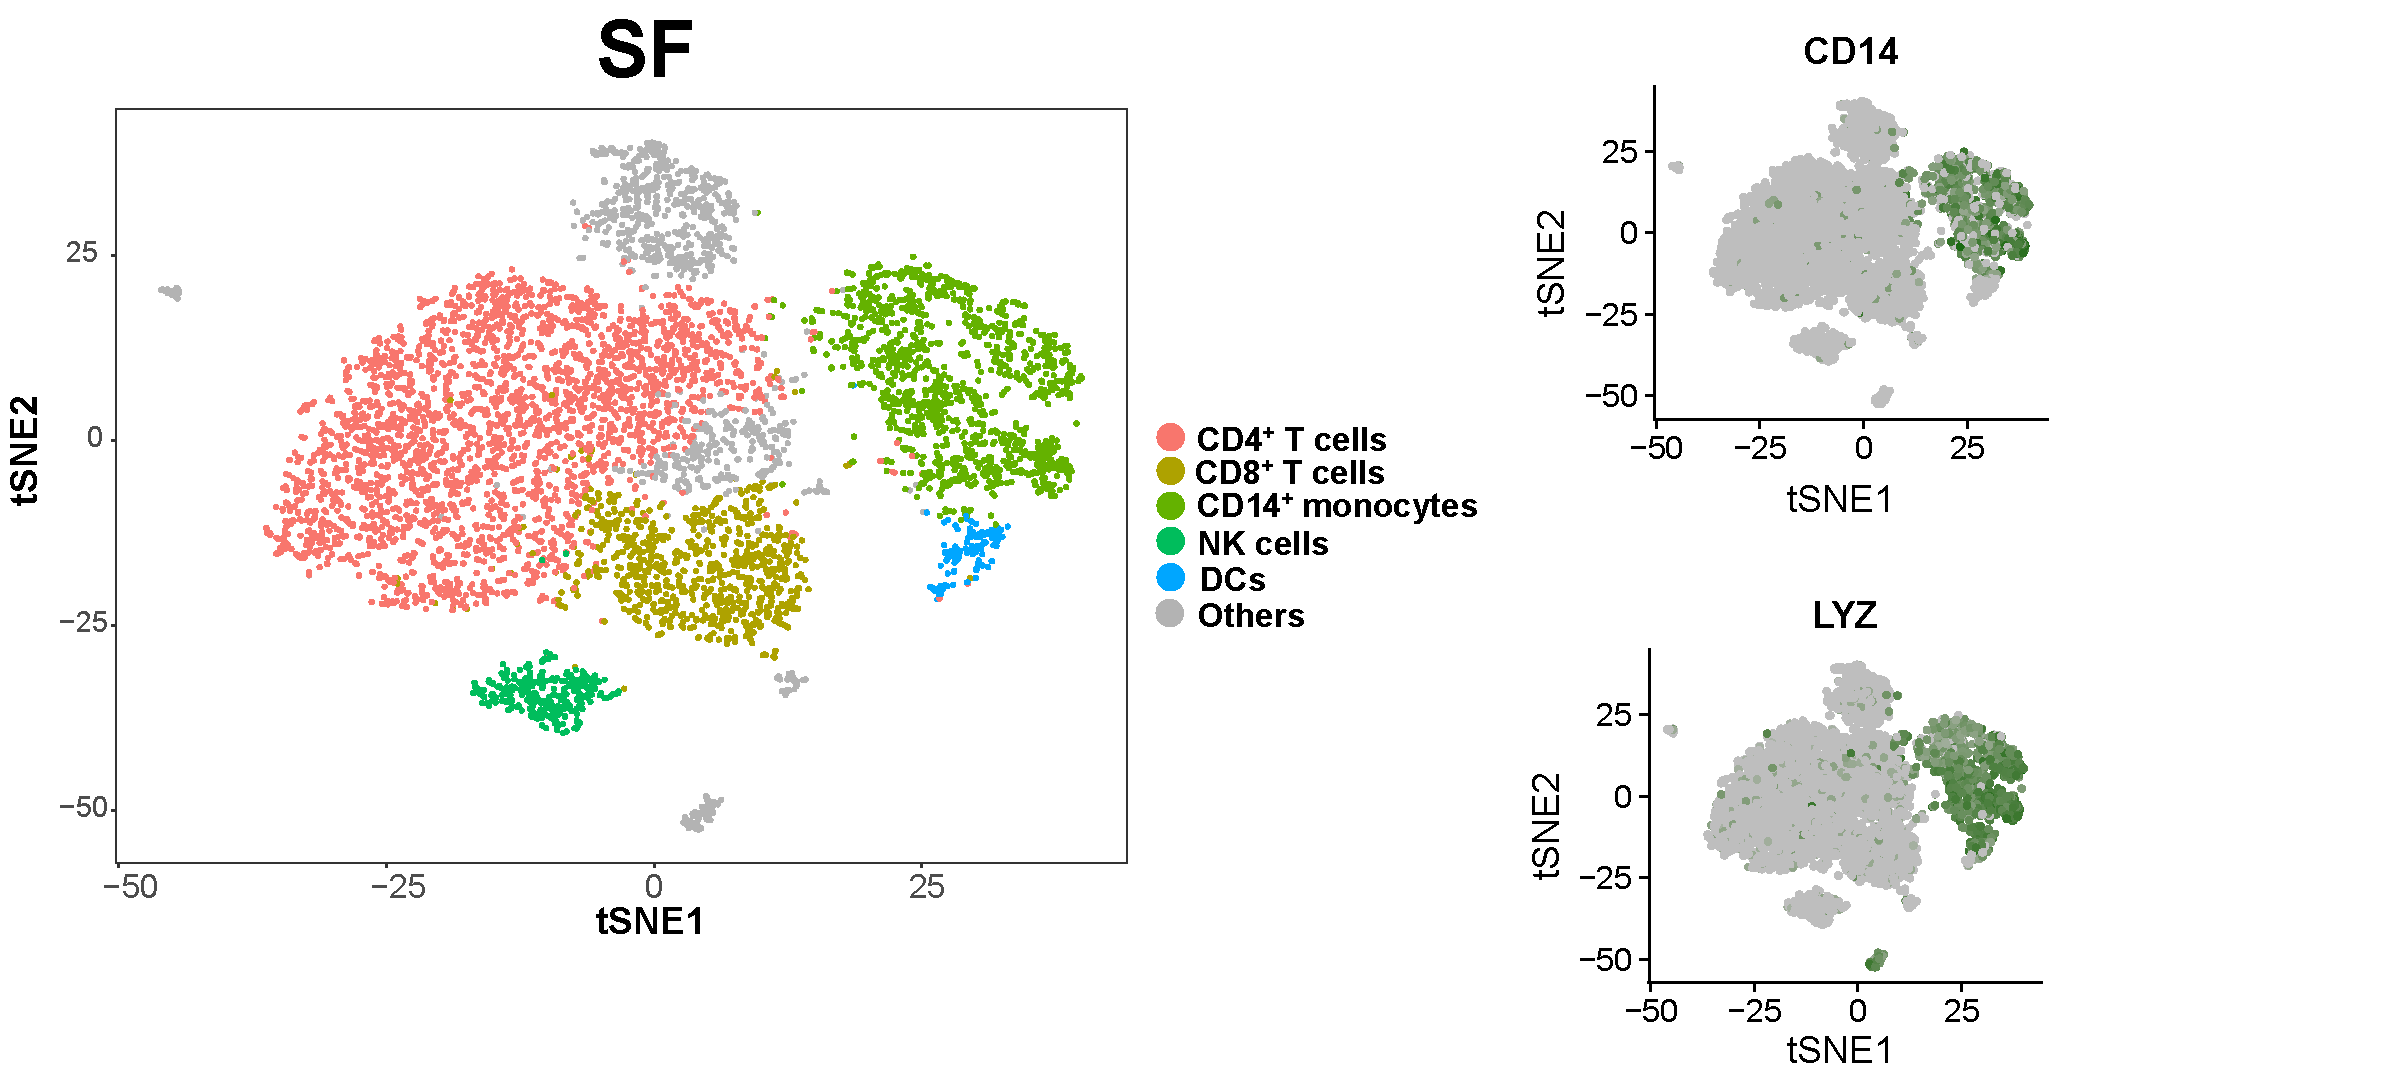
\includegraphics[width=\textwidth]{./Appendix/pdfs/Chapter5/PSA_SF_clusters_and_monocytes_markers}
\caption{}
\end{subfigure}
~
\begin{subfigure}[b]{0.70\textwidth} 
%the [b] prevents offset in subcaptions
\centering
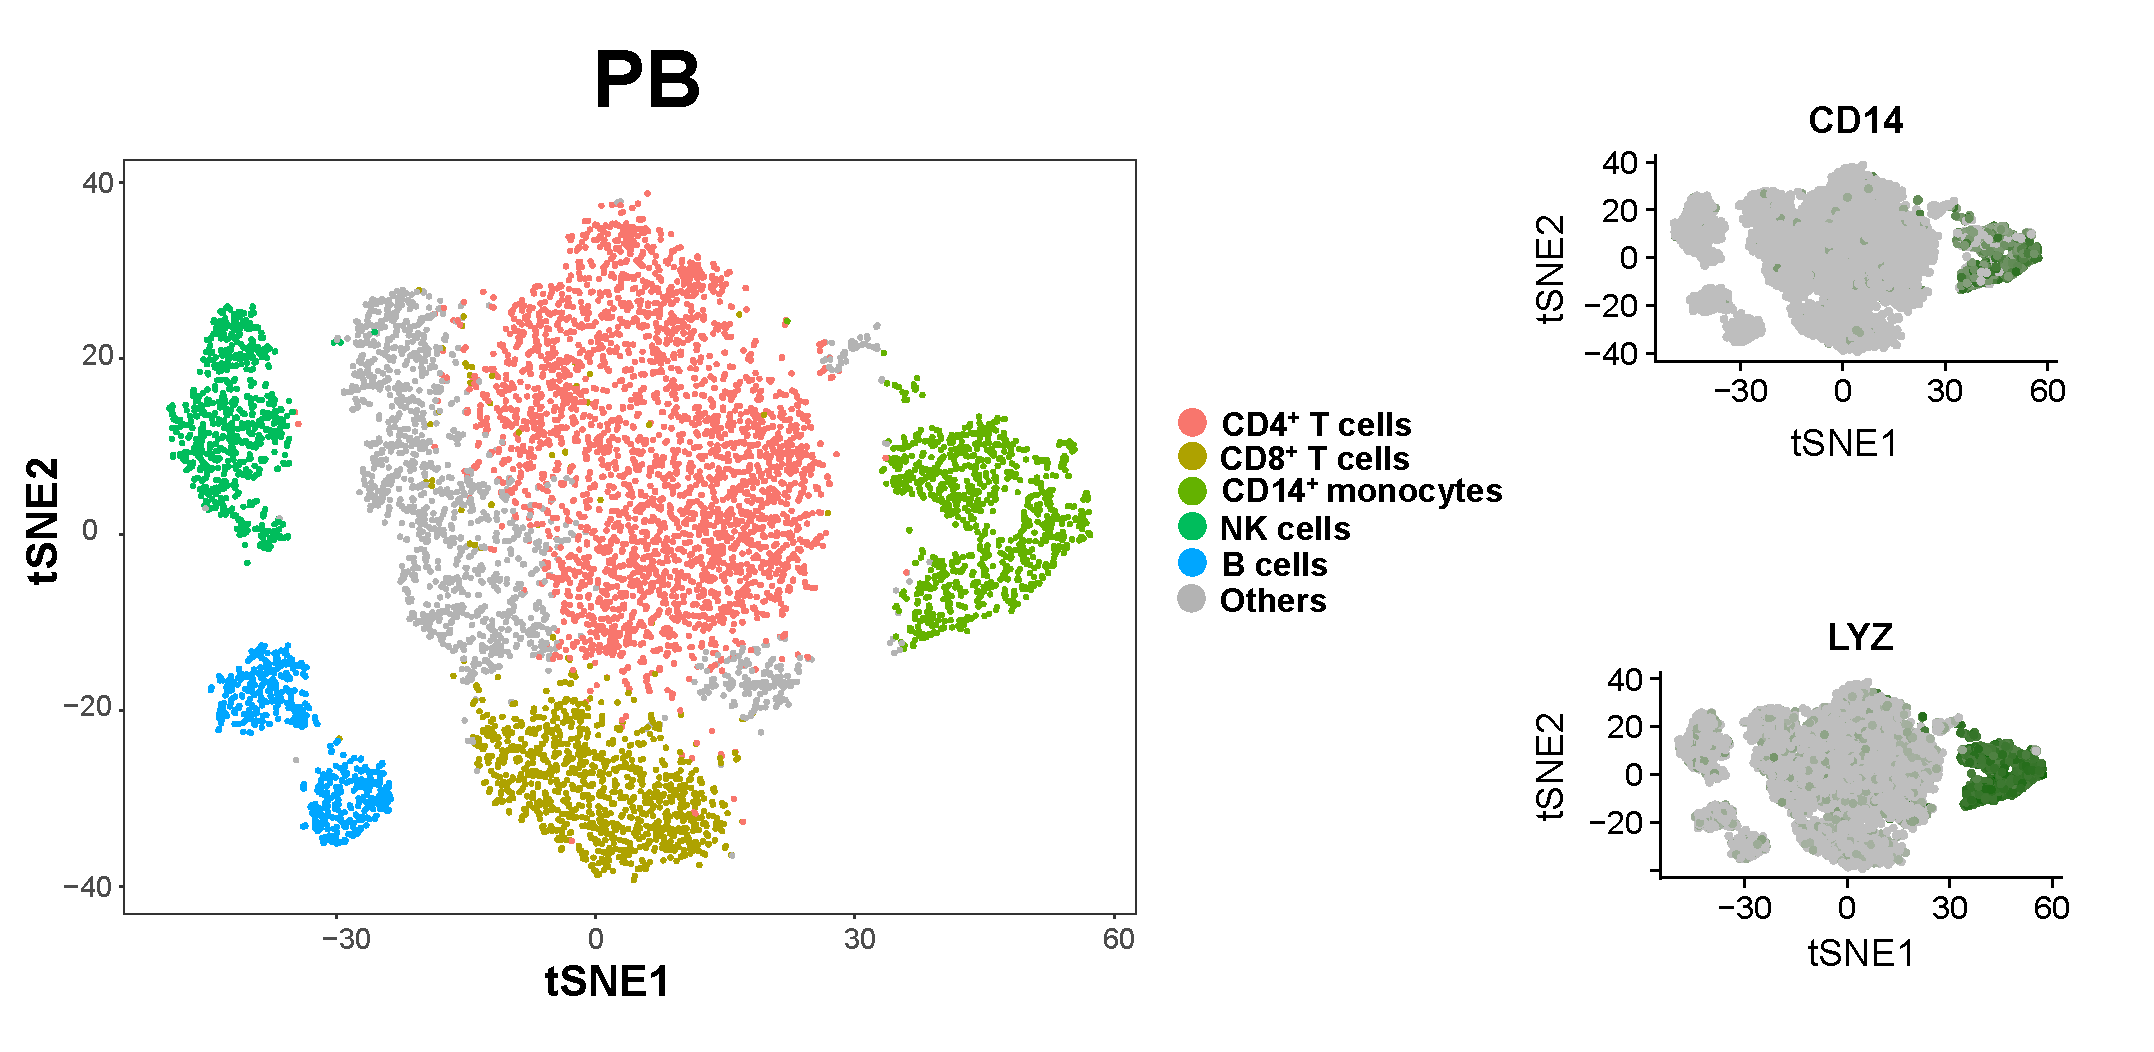
\includegraphics[width=\textwidth]{./Appendix/pdfs/Chapter5/PSA_PB_clusters_and_monocytes_markers}
\caption{}
\end{subfigure}
\caption[Identification of the CD14$^+$ monocytes populations from bulk SFMCs and PBMCs using scRNA-seq transcriptomes.]{\textbf{Identification of the CD14$^+$ monocytes populations from bulk SFMCs and PBMCs using scRNA-seq transcriptomes.} xxxx}
\label{figure:PsA_scRNAseq_SF_an_PB_monocytes_identification_from_bulk}
\end{figure}